\documentclass{article}

\usepackage{tikz,tcolorbox}
\usepackage{graphicx} % Required for inserting images
\usepackage{amssymb}
\usepackage{amsmath}
\usepackage{marginnote}
\usepackage{amsthm}

\usepackage{hyperref}
\usepackage{lastpage}
\usepackage{fancyhdr}
\usepackage{geometry}
\geometry{margin=1in}
\usepackage{underscore}
\usepackage{subcaption}
\usepackage{fancyvrb}
\usepackage{listings}
\lstset{
basicstyle=\small\ttfamily,
columns=flexible,
breaklines=true
}
\usepackage{tabularx}
\usepackage{float}
\usepackage{makecell}

\newtheorem*{theorem}{Theorem}
\newtheorem*{definition}{Definition}
\theoremstyle{definition}
\newtheorem*{example}{Example}\theoremstyle{definition}
\newtheorem*{nonexample}{Non-Example}

\title{Math111a: Abstract Algebra notes}
\author{Mann Malviya}
\date{Fall 2024}

\begin{document}

\maketitle

\section*{Lecture 1}
The 3 main pillars of modern mathematics,
\begin{figure}[H]
	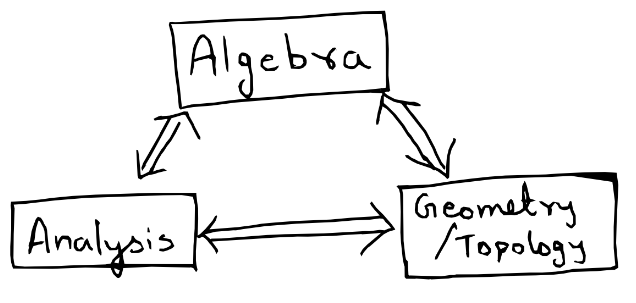
\includegraphics[scale=2]{3main_pillars.png}
\end{figure}

Some of the features of math which distinguishes it from other areas of knowledge,
\begin{itemize}
    \item proof (objective truth)
    \item axiomatization (the axiomatic approach)
    \item abstraction
\end{itemize}

\noindent These are very well exemplified in the study of Algebra(A.K.A Abstract Algebra).

\

\noindent"Abstract Algebra":Study of various different  kinds of "algebraic structures".

\noindent\textbf{Eg:} $\underbrace{\text{groups}}_{\text{Math 111a}}$, 
$\underbrace{\text{rings, fields}}_{\text{Math 111b}}$, $\underbrace{\text{vector spaces}}_{\text{Math 117}}$, modules, algebras.

\

Each kind of algebraic structure is axiomatized: A set + some operations subject to some axioms.

\

\noindent This Course: Group Theory

\subsection*{Chapter I: Fundamentals}

\subsubsection*{\underline{\S (I.1) The definition of a group}}
\begin{tcolorbox} [title= Definition:, colback=black!10!white]
    A \underline{binary operation}(or law of composition) on a set S is a rule which assigns to any pair of elements of S a third element of S. More formally it is a function.
    $$m:S\times S\to S$$
    $$(a,b)\mapsto m(a,b)$$
    where $S\times S=\{(a,b)|a,b\in S\}$ is the set of ordered pairs of elements of $S$. It maps an ordered pair $(a,b)$ to some element $m(a,b)\in S$.
\end{tcolorbox}


\begin{example}
    Addition defines a binary operation on the set $\mathbb{Z}$ of integers.
    $$\mathbb{Z}\times\mathbb{Z}\to\mathbb{Z}$$
    $$(a,b)\mapsto a+b$$
\end{example}

\begin{example}
    Multiplication also defines a binary operation on $\mathbb{Z}$.
    $$\mathbb{Z}\times\mathbb{Z}\to\mathbb{Z}$$
    $$(a,b)\mapsto ab$$
    There are many more examples of a similar nature.
\end{example}

\begin{example}
    Multiplication also defines a binary operation on the set $\mathbb{Z}^+$.
    $$\mathbb{Z}^+\times\mathbb{Z}^+\to\mathbb{Z}^+$$
    $$(a,b)\mapsto ab$$
\end{example}

\begin{nonexample}
    Multiplication does not define a binary operation on the set $\mathbb{Z}^-$. Easy way to see this is, 
    $$((-1)(-2)=+2)$$
\end{nonexample}

\begin{example}
    Addition of matrices defines a binary operation on the set $M_{m\times n}(\mathbb{R})$ of all $m\times n$ matrices with real entries.
    $$M_{m\times n}(\mathbb{R})\times M_{m\times n}(\mathbb{R})\to M_{m\times n}(\mathbb{R})$$
    $$(A,B)\mapsto A+B$$
\end{example}

\begin{example}
    Multiplication of matrices defines a binary operation on the set $M_n(\mathbb{R})$ of square $n\times n$ matrices with real entries.
    $$M_n(\mathbb{R})\times M_n(\mathbb{R})\to M_n(\mathbb{R})$$
    $$(A,B)\mapsto AB$$

    Note that $AB\neq BA$ in general, For example, take $n=2$,
    $$A=\left(\begin{array}{cc}
        1&1\\
        0&0
    \end{array}\right) \ \& \ B=\left(\begin{array}{cc}
        0&1\\
        0&1
    \end{array}\right)$$

    $$AB=\left(\begin{array}{cc}
        1&1\\
        0&0
    \end{array}\right)\left(\begin{array}{cc}
        0&1\\
        0&1
    \end{array}\right)=\left(\begin{array}{cc}
        0&2\\
        0&0
    \end{array}\right)$$

    $$BA=\left(\begin{array}{cc}
        0&1\\
        0&1
    \end{array}\right)\left(\begin{array}{cc}
        1&1\\
        0&0
    \end{array}\right)=\left(\begin{array}{cc}
        0&0\\
        0&0
    \end{array}\right)$$
    we can clearly see, $AB\neq BA$.\\
    Thus a binary operation $m:S\times S\to S$ need not be commutative. We can have $m(a,b)\neq m(b,a)$. The order can matter. This shouldn't be too hard to believe as in the case of ordered pairs, $(a,b)\neq(b,a)$ unless $a=b$
\end{example}
\begin{tcolorbox} [title= Definition:, colback=black!10!white]
    A \underline{group} is a set $G$ equipped with a binary operation.
    $$G\times G\to G$$
    $$(a,b)\mapsto ab$$
    Such that the following axioms hold:
    \begin{enumerate}
        \item[(1)] The group operation is associative, i.e.,
        $$(ab)c=a(bc) \ \ \forall a,b,c\in G$$
        \item[(2)] There exits an element $e$ in $G$ such that,
        $$ea=a=ae \ \ \forall a\in G$$ 
        \item[(3)] For every $a$ in $G$, there exists an element $a^{-1}$ in $G$ such that,
        $$aa^{-1}=e=a^{-1}a$$
    \end{enumerate}
\end{tcolorbox}


\noindent\underline{Remark:}
\begin{itemize} 
    \item The element $e$ in axiom (2) is \underline{unique}.\\
Indeed, suppose $e'$ were another element satisfying, $e'a=a=ae',\ \ \forall a\in G$.
$$e\underset{(2)\text{ for e'}}{=}ee'\underset{(2)\text{ for e}}{=}e$$
This unique element of the group is called the \underline{identity element} of the group.

    \item The element $a^{-1}$ in Axiom (3) is also unique and called the \underline{inverse} of a.\\
    Suppose $a'$ were an element such that $aa'=e=a'a$
    $$a^{-1}\underset{(2)}{=}a^{-1}e\underset{(3)\text{ for a'}}{=}a^{-1}(aa')\underset{(1)}{=}(a^{-1}a)a'\underset{(3)\text{ for a}}{=}ea'\underset{(2)}{=}a'$$

    In a sentence: "A group is a set equipped with an associative binary operation which has an identity element and in which every element has an inverse."
    \item Axiom (3) is probably the most significant of the axioms because it distinguishes the notion of a group from many other algebraic structures.\\
    "It implies that in a group, multiplying by any element can be "undone""
    $$a\leadsto ab\leadsto (ab)b^{-1}=a(bb^{-1})=ae=a$$
    \item The associativity axiom is common but important. However, there do exist non-associative operations in math.\\
    \underline{Example:} The cross product $\vec{v}\times\vec{w}$ of vectors in 3-dimensions Euclidean space defines a non-associative binary operation in $\mathbb{R}^3$(see the exercises).
    \item Suppose we have an ordered sequence $a_1,a_2,...,a_n$ in a group $G$ that we would like to multiply together. There will be many ways of doing this by successively multiplying pairs of elements together.\\
    \underline{For Example:} There are 2 ways of multiplying together a sequence of n=3 elements a,b,c.
    $$a(bc)$$
    $$(ab)c$$
    Axiom (1) asserts that the result is the same,
    $$(ab)c=a(bc)$$
    On the other hand there are 5 ways of multiplying n=4 elements together, a,b,c,d.
    $$((ab)c)d$$
    $$(a(bc))d$$
    $$(ab)(cd)$$
    $$a((bc)d)$$
    $$a(b(cd))$$
    One can show using Axiom (1) that they all coincide.\\
    \noindent Eg: \begin{eqnarray*}
        ((ab)c)d&= (a(bc))d\\
        &=a((bc)d)\\
        &=a(b(cd))
    \end{eqnarray*}
\end{itemize}

\begin{theorem}
    (The Generalized Associativity Law) The result of multiplying together an ordered sequence of elements in a group does not depend on the choice of bracketing.
\end{theorem}

The proof of this Theorem is a very tedious inductive argument which can be found in books.

\noindent \underline{Remark:} The generalized associativity law allows us to speak of the element.
$$a_1a_2...a_n\in G$$
Without specifying brackets.

\noindent\textbf{Exercise:}
Show:
\begin{itemize}
    \item $e^{-1}=e$
    \item $(ab)^{-1}=b^{-1}a^{-1}$
    \item $(a_1a_2...a_n)^{-1}=a_n^{-1}a_{n-1}^{-1}...a_2^{-1}a_1^{-1}$
\end{itemize}

\textit{\underline{hint}: Use the property that the inverse element is unique. The 3rd exercise requires Induction.}

\noindent\underline{Remark:} For any element $a$ in a group $G$, we define,
$$a^0=e$$
$$a^1=a$$
$$a^2=a\cdot a$$
$$:$$
$$a^n=a(a^{n-1})=\underbrace{aa...a}_{\text{n times}}$$ for any $n\ge1$.

Also we define,
$$a^{-n}=(a^{-1})^n=(a^n)^{-1}$$
for any $n\ge1$.

Thus we have a well-defined element $$a^n\in G$$ 
for every integer $n\in\mathbb{Z}$

\begin{tcolorbox} [title= Definition:, colback=black!10!white]
    Let $a$ be an element in a group $G$. If there is some integer $n\ge1$ such that $a^n=e$, then $a$ is an element of \underline{finite order}. Otherwise, $a$ is an element of \underline{infinite order}.
    $$...\ a^{-2}\ \ a^{-1}\ \ a^0=e\ \ a^1=a\ \ a^2\ \ a^3...$$
\end{tcolorbox}

\noindent\textbf{Exercise:} Prove: 
$$a^n=e \ \ \ \text{iff}\ \ \ a^{-n}=e$$

The \underline{order} of $a$ is the least +ve integer $n$ such that $a^n=e$, or $\infty$ if there is no such $n$.

\noindent\underline{Example:} $e$ is the unique element of order 1.

\begin{tcolorbox} [title= Definition:, colback=black!10!white]
    A group $G$ is \underline{finite} if it has finitely many elements. Otherwise $G$ is infinite. \\
    The order of a group $G$(either finite or infinite) is its cardinality, i.e., the number of elements in $G$. We write $|G|$ for the order of $G$.
\end{tcolorbox}

\begin{tcolorbox} [title= Definition:, colback=black!10!white]
    A group $G$ is said to be \underline{abelian} (or \underline{commutative}) if $ab=ba,\ \ \ \forall a,b\in G$
\end{tcolorbox}
In general, we say that two elements $a,b\in G$ commute if $ab=ba$.

\subsubsection*{\underline{\S (I.2) Examples}}
\noindent\underline{Example:} The set $G=\{e\}$ which has a single element with the only one possible multiplication is a group. It is called the trivial group(a unique group with order 1).

\noindent\underline{Remark:} If $G=\{a_1,a_2,...,a_n\}$ is a finite group, then we can completely specify the group operation by writing down a multiplication table.
\begin{table}[H]
    \centering
    \begin{tabular}{c|cccc}
        xy & $a_1$ & $a_2$ & ...& $a_n$\\
        \hline
        $a_1$ & $a_1a_1$ & $a_1a_2$ & ...& $a_1a_n$\\
        $a_2$ & $a_2a_1$ & $a_2a_2$ & ...&$a_2a_n$\\
        : & & :& &:\\
        $a_n$&&...&& $a_na_n$
    \end{tabular}
\end{table}

\noindent\underline{Example:} Let $G=\{e,a\}$ be the 2-element set with multiplication table.
\begin{table}[H]
    \centering
    \begin{tabular}{c|cc}
        & $e$ & $a$\\
        \hline
        $e$ & $ee$ & $ea$\\
        $a$ & $ae$ & $aa=e$
    \end{tabular}
\end{table}
This table can be simplified and written as,
\begin{table}[H]
    \centering
    \begin{tabular}{c|cc}
        & $e$ & $a$\\
        \hline
        $e$ & $e$ & $a$\\
        $a$ & $a$ & $e$
    \end{tabular}
\end{table}
This is a group of order 2.

\noindent\underline{Example:} Let $G=\{+1,-1\}$ with ordinary multiplication.
\begin{table}[H]
    \centering
    \begin{tabular}{c|cc}
        & $+1$ & $-1$\\
        \hline
        $+1$ & $+1$ & $-1$\\
        $-1$ & $-1$ & $+1$
    \end{tabular}
\end{table}
This is essentially the same group as the previous example, we have just labelled things differently.

\noindent\underline{Example:} Let $G=\{e,a,b\}$ with
\begin{table}[H]
    \centering
    \begin{tabular}{c|ccc}
        & $e$ & $a$ & $b$\\
        \hline
        $e$ & $e$ & $a$ & $b$\\
        $a$ & $a$ & $b$ & $e$\\
        $b$ & $b$ & $e$ & $a$
    \end{tabular}
\end{table}
Is a group of order $3$.

Saying a group is abelian is same as saying multiplication table is symmetric about the diagonal.

\ 

\noindent\textbf{Exercise:} The multiplication table for a finite group must be a \underline{latin square}, i.e., every element appears exactly once in each row and column.

\noindent\underline{Example:} $G=\{e,a,b,c\}$. The following are 2 groups of order 4:
\begin{table}[H]
    \centering
    \begin{tabular}{c|cccc}
        $G_1$ & $e$ & $a$ & $b$ & $c$\\
        \hline
        $e$ & $e$ & $a$ & $b$ & $c$\\
        $a$ & $a$ & $b$ & $c$ & $e$\\
        $b$ & $b$ & $c$ & $e$ & $a$\\
        $c$ & $c$ & $e$ & $a$ & $b$
    \end{tabular}
\end{table}

\begin{table}[H]
    \centering
    \begin{tabular}{c|cccc}
        $G_1$ & $e$ & $a$ & $b$ & $c$\\
        \hline
        $e$ & $e$ & $a$ & $b$ & $c$\\
        $a$ & $a$ & $e$ & $c$ & $b$\\
        $b$ & $b$ & $c$ & $e$ & $a$\\
        $c$ & $c$ & $b$ & $a$ & $e$
    \end{tabular}
\end{table}

$$G_1=\langle a|a^4\rangle$$
$$G_2=\langle a,b|a^2,b^2,[a,b]\rangle$$

\begin{center}
	\line(1,0){450}
\end{center}

\section*{Lecture 2}

\end{document}
